\section{Численные методы решения обыкновенных дифференциальных уравнений}

\subsection{Решение задачи Коши для ОДУ второго порядка}

\subsubsection{Постановка задачи}
Реализовать методы Эйлера, Рунге-Кутты и Адамса 4-го порядка в виде программ, задавая в качестве входных данных шаг сетки $h$. С использованием разработанного программного обеспечения решить задачу Коши для ОДУ 2-го порядка на указанном отрезке. Оценить погрешность численного решения с использованием метода Рунге – Ромберга и путем сравнения с точным решением.

{\bfseries Вариант:}
\begin{multline*}
y'' + y - 2\cos{x} = 0 \\
y(0) = 0 \\
y'(0) = 1 \\
x \in [0, 1],\ h = 0.1 \\
\textup{Точное решение: }y = x\sin{x} + \cos{x} \\
\end{multline*}

\subsubsection{Результаты работы}
\begin{alltt}
$ cat tests/1/1.txt
0 1
1
0
0.1
$ ./lab4_1 < tests/1/1.txt
Метод Эйлера:
1 1.005 1.01988 1.04418 1.07717 1.11783 1.16488 1.21681 1.27188 1.32817 1.38362
Погрешность: 0.00181351

Метод Рунге-Кутты:
1 1.00499 1.0198 1.04399 1.07683 1.1173 1.16412 1.21579 1.27059 1.3266 1.38177
Погрешность: 1.11895e-06

Метод Адамса:
1 1.00499 1.0198 1.04399 1.07683 1.11729 1.16412 1.2158 1.27059 1.32661 1.38178
Погрешность: 1.60996e-06
\end{alltt}

\begin{figure}[h]
\centering
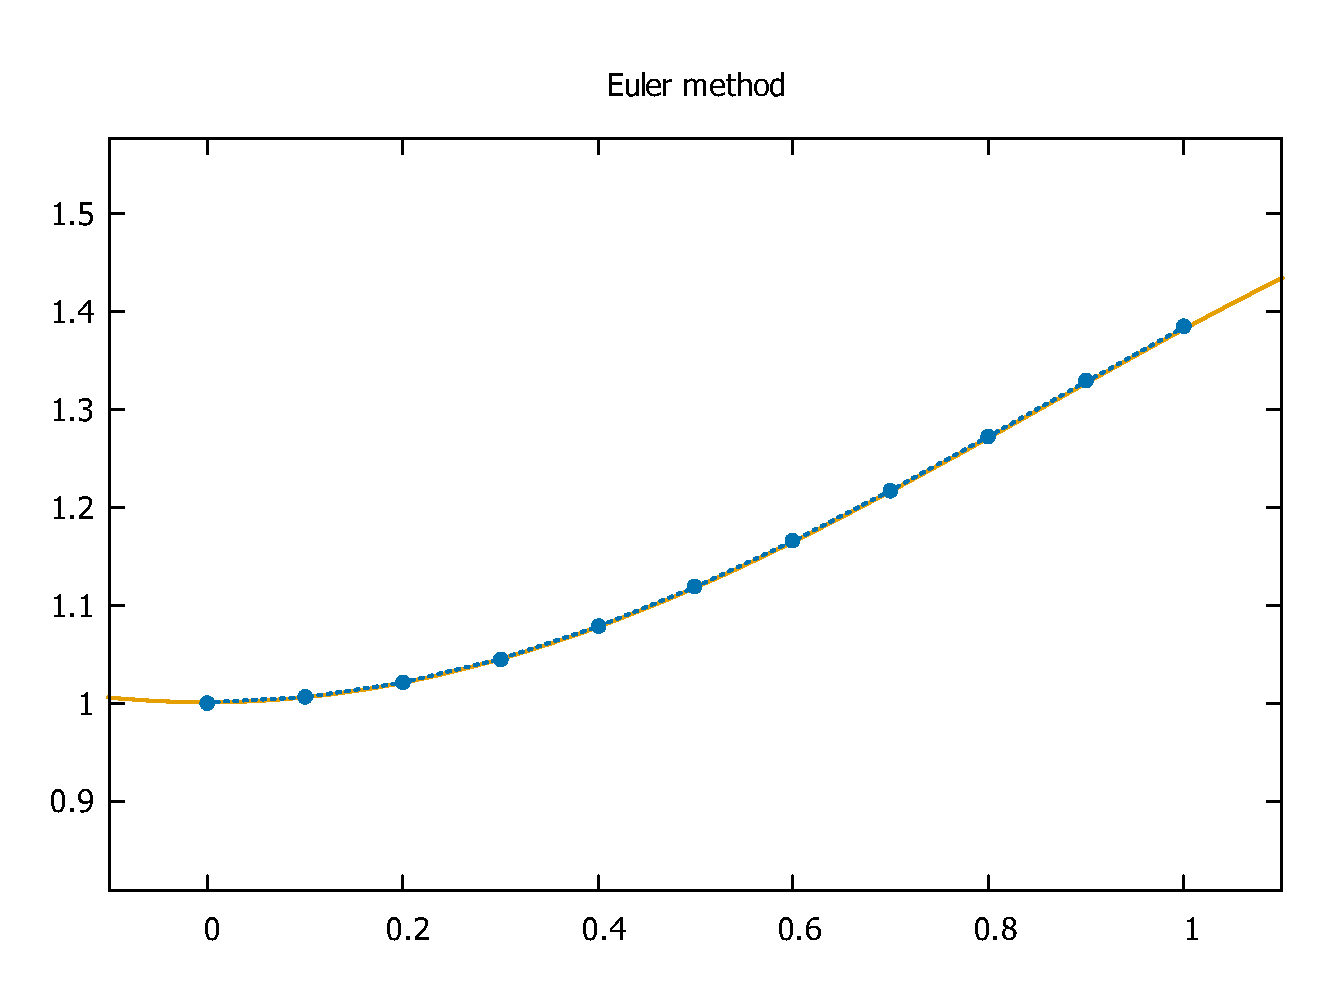
\includegraphics[height=.33\textheight]{lab4_1_euler}
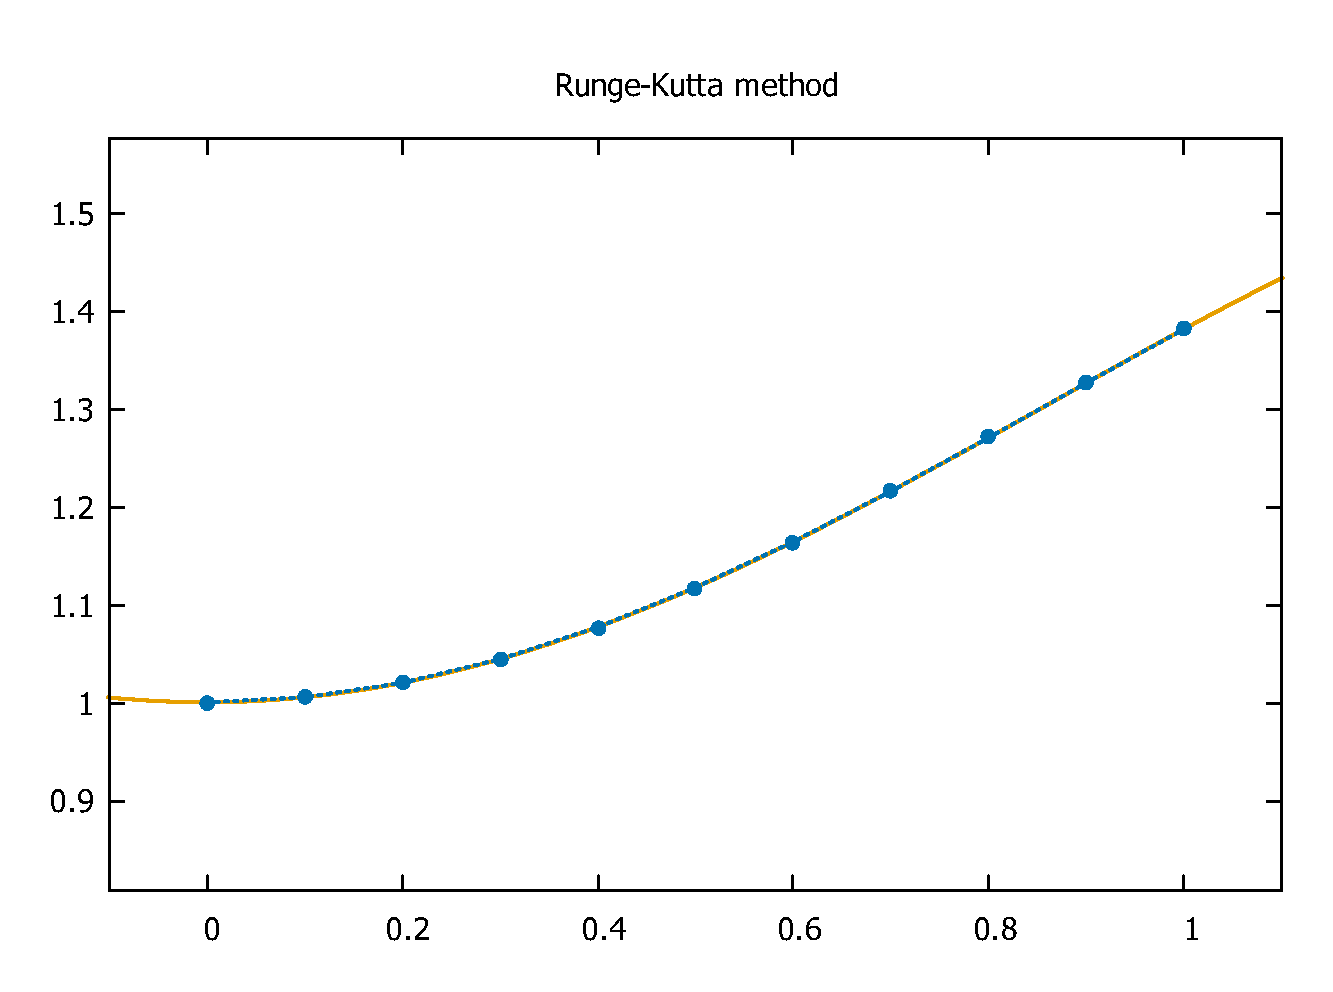
\includegraphics[height=.33\textheight]{lab4_1_runge_kutta}
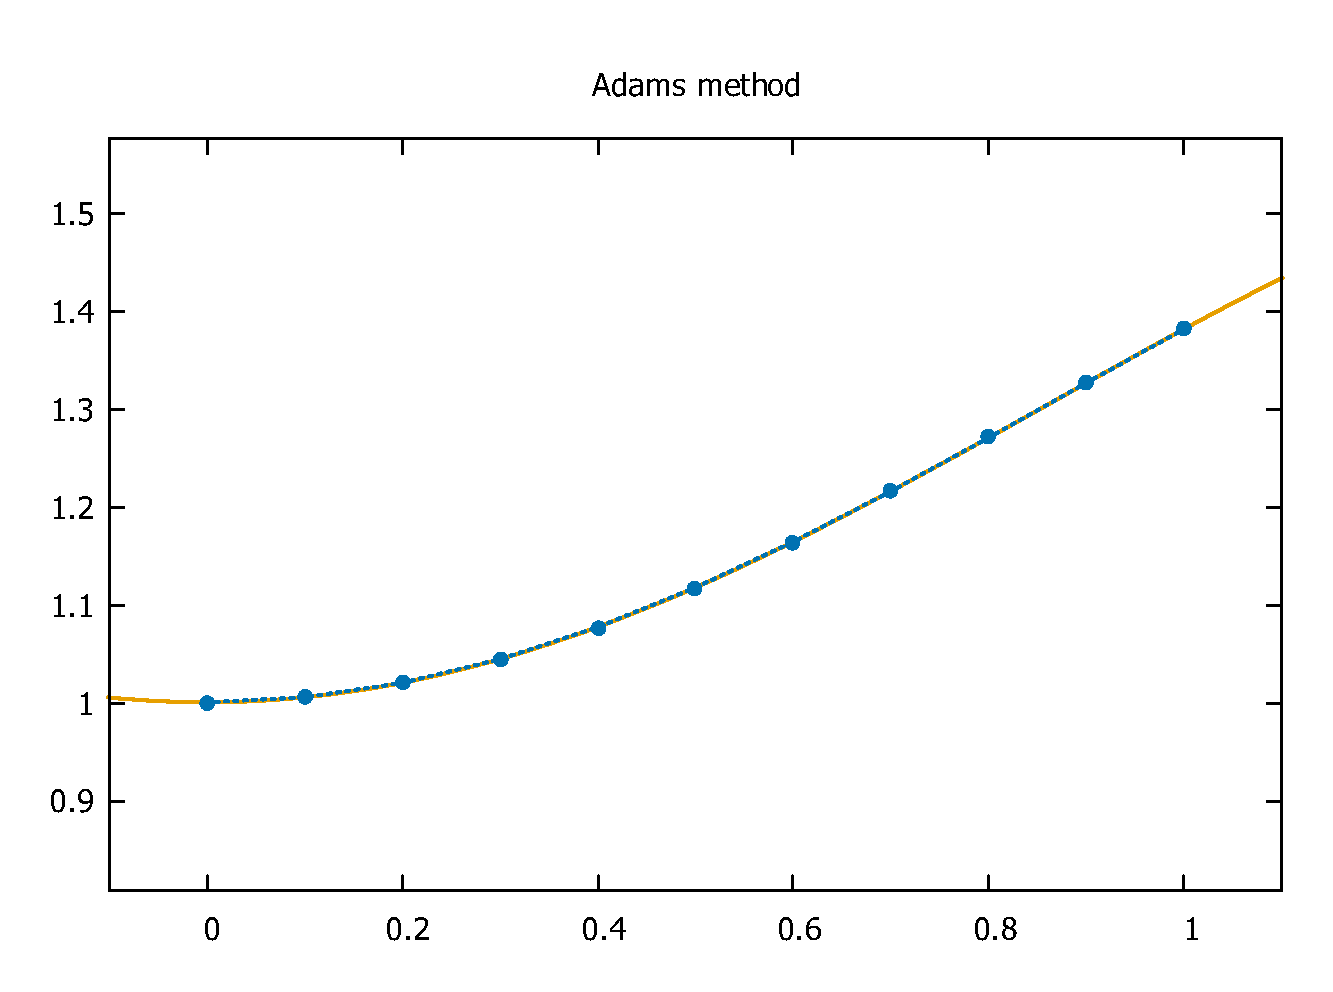
\includegraphics[height=.33\textheight]{lab4_1_adams}
\end{figure}
\FloatBarrier
\pagebreak

\subsubsection{Исходный код}
\lstinputlisting{../include/differential/cauchy_problem.hpp}
\pagebreak

\subsection{Решение краевой задачи для ОДУ второго порядка}

\subsubsection{Постановка задачи}
Реализовать метод стрельбы и конечно-разностный метод решения краевой задачи для ОДУ в виде программ. С использованием разработанного программного обеспечения решить краевую задачу для обыкновенного дифференциального уравнения 2-го порядка на указанном отрезке. Оценить погрешность численного решения с использованием метода Рунге – Ромберга и путем сравнения с точным решением.

{\bfseries Вариант:}
\begin{multline*}
xy'' + 2y' - xy = 0 \\
y(1) = e^{-1} \\
y(2) = 0.5 e^{-2} \\
\textup{Точное решение: }y = \frac{e^{-x}}{x} \\
\end{multline*}

\subsubsection{Результаты работы}
\begin{alltt}
0.1
Метод стрельбы:
0.367879 0.302612 0.250998 0.209643 0.176143 0.148756 0.126187 0.107462 0.0918336 0.0787208 0.0676676
Погрешность: 1.69614e-05

Метод конечных разностей:
0.367879 0.302618 0.251008 0.209655 0.176156 0.148768 0.126198 0.107471 0.0918396 0.0787239 0.0676676
Погрешность: 1.51834e-05
\end{alltt}

\begin{figure}[h]
\centering
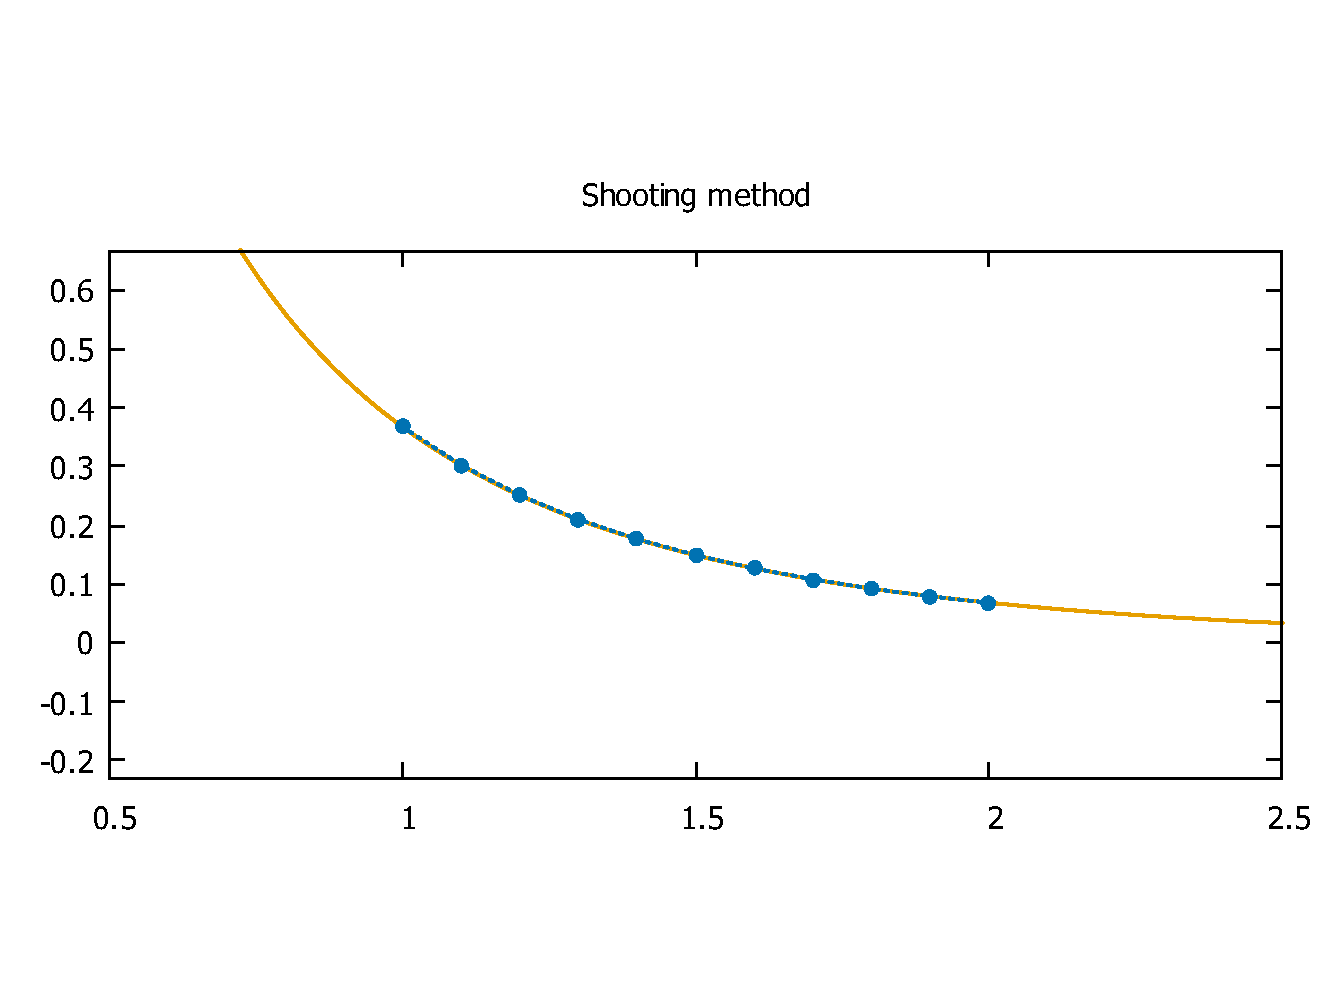
\includegraphics[height=.5\textheight]{lab4_2_shooting}
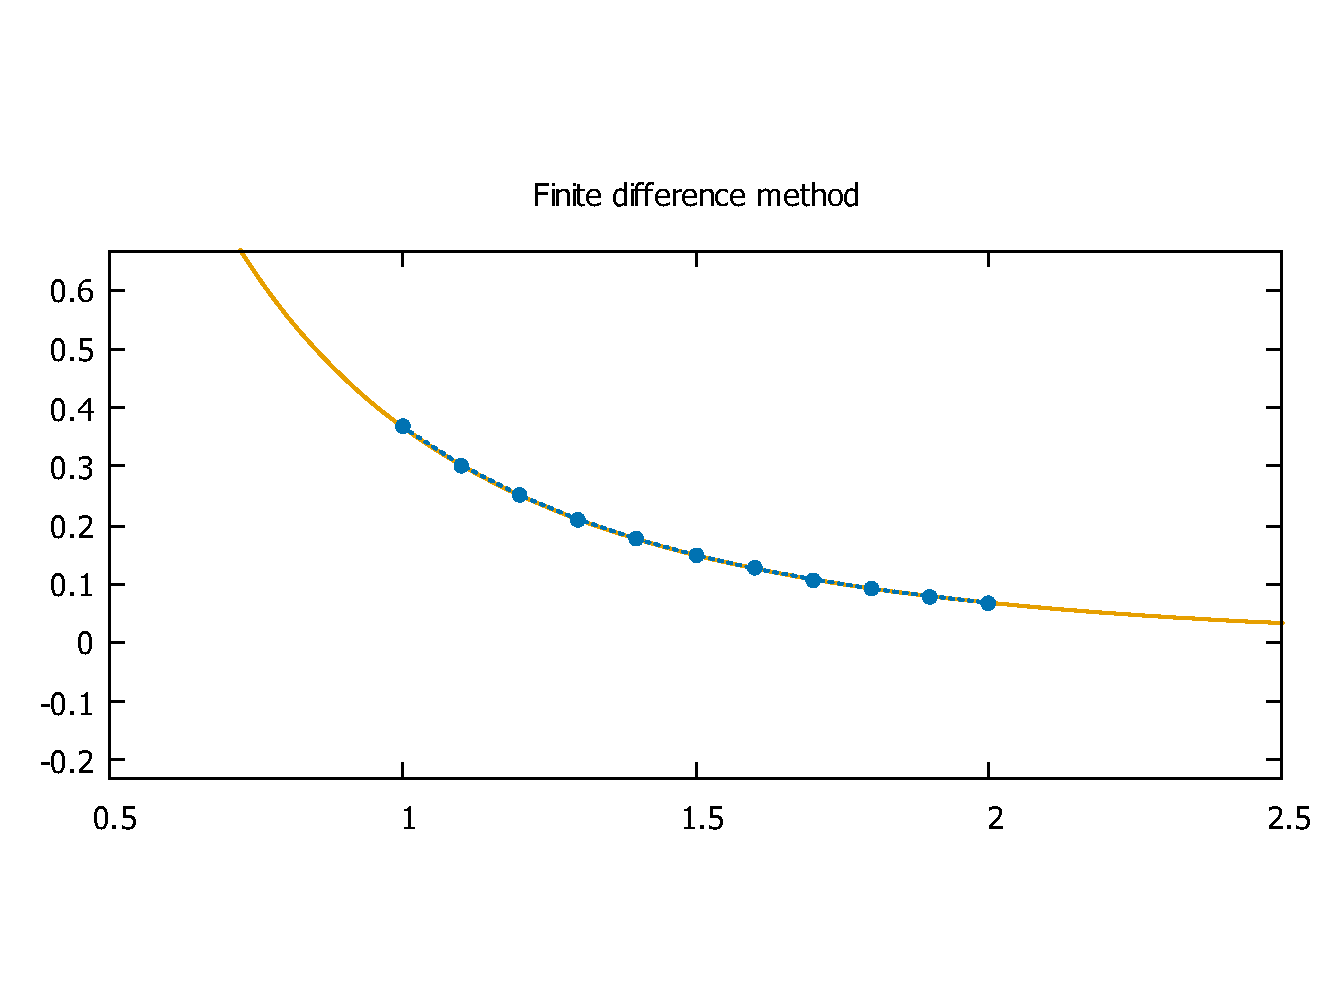
\includegraphics[height=.5\textheight]{lab4_2_finite_difference}
\end{figure}
\FloatBarrier
\pagebreak

\subsubsection{Исходный код}
\lstinputlisting{../include/differential/boundary_value_problem.hpp}
\pagebreak